% METHODS

The LED sample with its metal layers shown in \autoref{fig:metal_layers} was grown by the staff of the course and given to the student group.
To form a working LED from the metal layer sample, the following steps were done at NTNU NanoLab:

\begin{enumerate}
    \item Front contact formation
    \item GaAs contact layer etch
    \item Backside contact formation
    \item Mesa etch, PECVD passivation deposition, and contact annealing
    \item Planarization and passivation layer etch
    \item Pad metallization
\end{enumerate}

\begin{figure}[h]
    \centering
    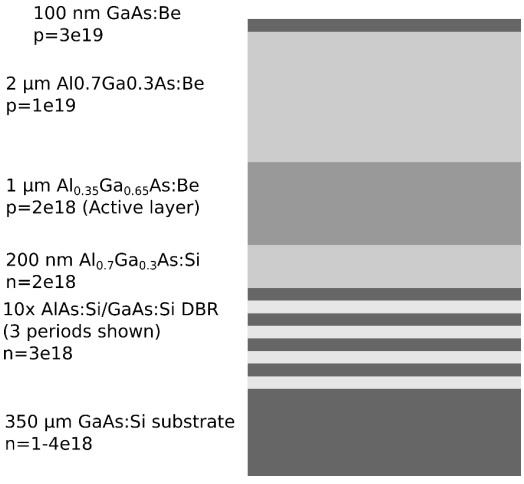
\includegraphics[width=0.45\textwidth]{figures/metal_layers.jpg}
    \caption{
        The metal layers the students got from the course staff to make the LED.
        The layers were grown in the MBE, molecular beam epitaxy, machine at NTNU NanoLab.
        Figure borrowed from the lab manual.
    }
    \label{fig:metal_layers}

\end{figure}

Each step was first done with a GaAs dummy sample to check that the process was working as intended.
After the last step, the LED was ready for testing at a lab at IES, the Department of Electronic Systems at NTNU.


\subsection{LED design}
\label{methods:led_design}

Different finger spacings and finger widths were tested.
An overview schematic of the LED design is shown in \autoref{fig:led_schematic}.
One LED was 1 mm x 1 mm.
The bus bar for contact pad was 1 mm x 40 \textmu m.
The bus bar connecting the fingers was 1 mm x 30 \textmu m.
The fingers were 500 \textmu m long, with widths at 4, 8, 12 and 16 \textmu m, and finger spacing at 40, 60, 80 and 100 \textmu m.
The second lithography layer was equal to the first, but scaled with a 5 \textmu m buffer everywhere to protect the fingers. 
The third lithography layer was for the mesa etch, and was a box around each LED with a 6 \textmu m buffer. 
The fourth lithography layer was for the etch of the passivation layer, and was just a 20 \textmu m x 980 \textmu m box on each bottom bus bar. 
The fifth and last lithography layer was for the etch of the pad metallization, and was a 900 \textmu m x 400 \textmu m box at the bottom of each LED connected to the bottom bus bar.
Schematics of the different layers are shown in \autoref{fig:CleWin_L1} to \autoref{fig:CleWin_L5}.
Schematics of the alignment marks in layer 1 and layer 2 is shown in \autoref{fig:CleWin_alignment_marks}.

% take in the figures on figures/CleWin_layer_figs.tex
% % clewin figures, L1 to L5 and alignment marks


% \begin{figure}[ht]
%     \centering
%     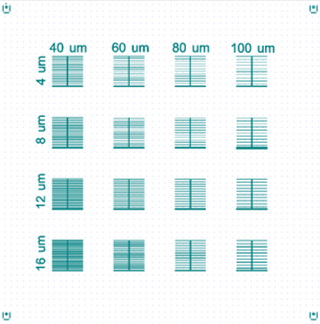
\includegraphics[width=0.45\textwidth]{figures/CleWin_L1.png}
%     \caption{
%         Layer 1. 
%         Numbers on the top is the width of the fingers in the matrix.
%         Numbers on the left side is the width of the fingers in the matrix.
%         Each LED is 1 mm x 1 mm. 
%     }
%     \label{fig:CleWin_L1}
% \end{figure}


% % L2
% \begin{figure}[ht]
%     \centering
%     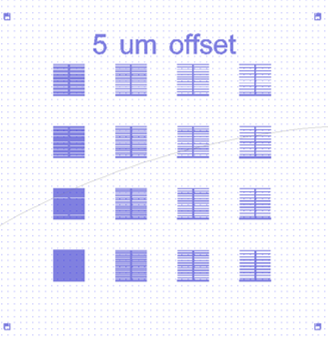
\includegraphics[width=0.45\textwidth]{figures/CleWin_L2.png}
%     \caption{
%         Layer 2. 
%         This is the same as layer 1, but with a 5 \textmu m buffer on the whole pattern. 
%     }
%     \label{fig:CleWin_L2}
% \end{figure}


% % L3 
% \begin{figure}[ht]
%     \centering
%     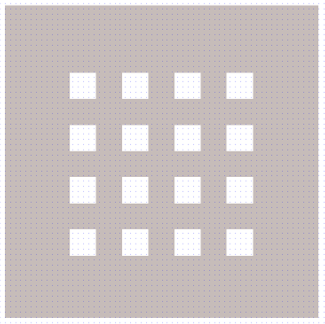
\includegraphics[width=0.45\textwidth]{figures/CleWin_L3.png}
%     \caption{
%         Layer 3. 
%         This is the mesa etch layer. 
%         The size of the box covering each LED is 1.012 mm x 1.012 mm.
%     }
%     \label{fig:CleWin_L3}
% \end{figure}

% % L4
% \begin{figure}[ht]
%     \centering
%     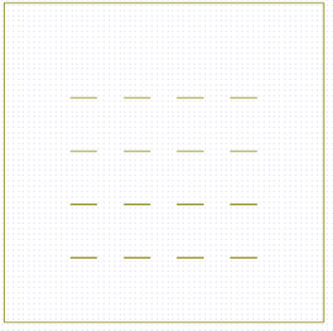
\includegraphics[width=0.45\textwidth]{figures/CleWin_L4.png}
%     \caption{
%         Layer 4. 
%         This is the HF etch layer. 
%         Each bar is covering a part of the bottom bus bar, with a size of 20 \textmu m x 980 \textmu m.
%     }
%     \label{fig:CleWin_L4}
% \end{figure}

% % L5
% \begin{figure}[ht]
%     \centering
%     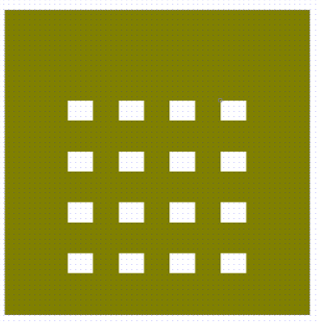
\includegraphics[width=0.45\textwidth]{figures/CleWin_L5.png}
%     \caption{
%         Layer 5. 
%         This is the pad metallization layer, where each box is 1 mm x 0.4 mm. 
%         The box is covering the bottom bus bar of each LED. 
%     }
%     \label{fig:CleWin_L5}
% \end{figure}


% % Alignment marks
% \begin{figure}[ht]
%     \centering
%     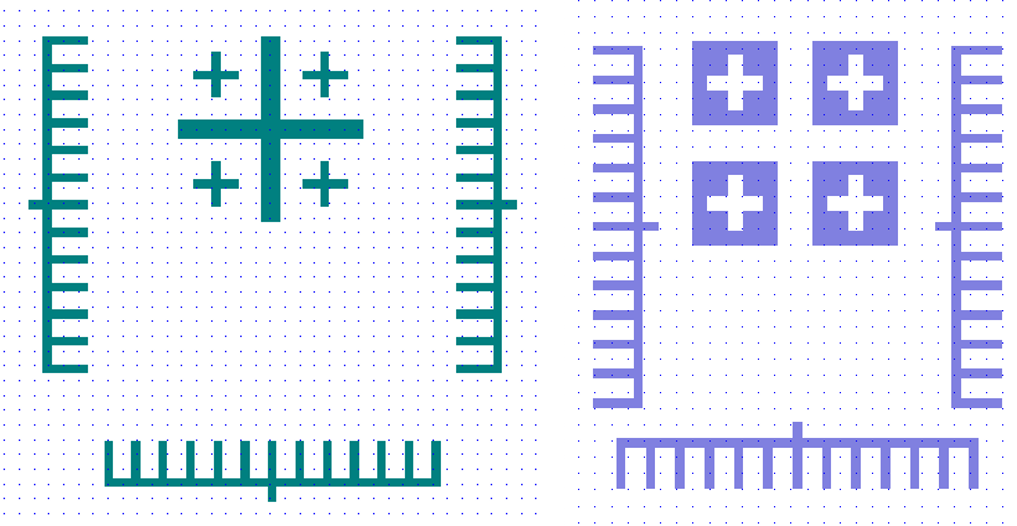
\includegraphics[width=0.45\textwidth]{figures/CleWin_alignment_marks.png}
%     \caption{
%         Alignment marks for layer 1 and 2. 
%         The design allows quantification of the alignment error.
%         These marks are the Verniers design. 
%     }
%     \label{fig:CleWin_alignment_marks}
% \end{figure}


\begin{figure}[ht]
    \centering
    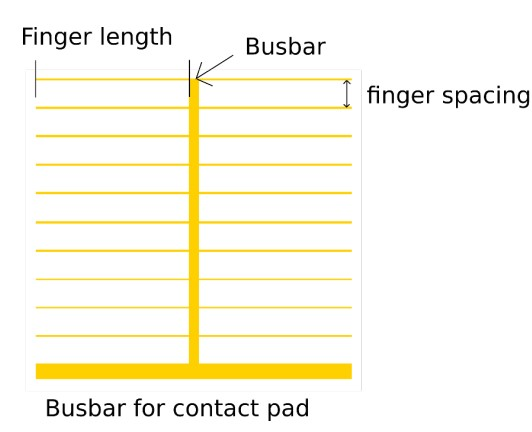
\includegraphics[width=0.45\textwidth]{figures/LED_schematic.jpg}
    \caption{
        Schematic of the LED design.
        Figure borrowed from the lab manual.
    }
    \label{fig:led_schematic}
\end{figure}


\subsection{Front contact formation}
\label{methods:front_contact}

The bus bar and its fingers were formed with lithography and lift-off.
A dose test was done to find the optimal dose and developing time for the resist, ensuring an undercut.
To verify this, both a SEM image and optical images of the sample were taken.
The optimal dose was 1300 mJ/cm$^2$ and the optimal developing time was 5 min.
All temperatures are probably some degrees off, since the hot plates at NanoLab havt not been calibrated for many years.
\textbf{FIX THESE NUMBERS}
Negative photoresist was used, and the steps were done in the following order:
\begin{enumerate}
    \item Cleaned the sample with acetone and IPA.
    \item Dehydration baked at 150 \textdegree C for 5 min.
    \item Spin coated MAN 440 resist at 4000 rpm for 30 s with 1000 rpm/s acceleration.
    \item Cleaned the backside.
    \item Soft baked at 95 \textdegree C for 1 min.
    \item Exposed the pattern at 1300 mJ/cm$^2$ in the MLA.
    \item Developed in maD-332S developer for 5 min.
    \item Optical inspected the pattern.
    \item Teaching assistants metallized the pattern with Au.
    \item Lift-off with acetone.
\end{enumerate}

Unfortunately, a mix up of the type of developer was done, and the lithography steps had to start over.
The optical inspection before round number two showed some bubbles on the wafer, which was probably caused by the wrong developer.
The wafer was cleaned thoroughly with acetone and IPA before the second round, but some residue might have been left behind.

Another problem was that the dose test were done with a resist that got emptied, and a newer resist had to be used for the actual process.
When using the new resist the developer time was increased from 5 to 6 minutes, which gave an undercut but damaged the alignment marks and the thinnest fingers.




\subsection{GaAs contact layer etch}
\label{methods:wet_etch}
The heavy p-doped GaAs layer at the top of the metal stack was etched away to allow light to pass through the LED.
The deposited Au fingers were measured to be 250 nm high in the profilometer.
Measuring the Au height was important for the later measurement of the etch depth of the 100 nm GaAs layer.
The Au fingers were protected with a positive photoresist before the wet etch.
Optimal dose for the positive photoresist was found to be 130 mJ/cm$^2$.
The preperation was done with the following steps:
\begin{enumerate}
    \item Cleaned the sample with IPA.
    \item Dehydration baked at 115 \textdegree C for 5 min.
    \item Spin coated SPR 700 resist at 4000 rpm for 34 s with 1000 rpm/s acceleration.
    \item Soft baked at 95 \textdegree C for 1 min.
    \item Aligned the pattern in the MLA. The alignment marks were badly damaged, so the alignment was not perfect. See \autoref{fig:align_marks}.
    \item Exposed the pattern at 130 mJ/cm$^2$ in the MLA.
    \item Post exposure baked at 115 \textdegree C for 1 min.
    \item Developed in maD-332S developer for 30 sec.
    \item Optical inspected the pattern to see if it covered the Au fingers.
\end{enumerate}

Quantification of the misalignment with the Verniers were tried, but the Verniers were too badly damaged to get any number out.
The wet etch was done at the chemical clanroom at NTNU NanoLab, with NH3:H2O2:H20 in 3:1:300 ratio.
The ammonium hydroxide was 30\%.
The etch depth was tested on the GaAs dummy sample, and measured with the profilometer to figure out an etch time which would remove 100 nm of GaAs.
The GaAs dummy was etched 50 nm at the first run, thus the time was doubled for the LED etch to achieve 100 nm.
The etch steps were as follows:

\begin{enumerate}
    \item All equipment and chemicals were placed in the fume hood.
    \item 3 mL 30\% NH$_3$ was added to the etch tank with 300 ml H$_2$O.
    \item 1 mL H$_2$O$_2$ was added to the etch tank.
    \item The sample was placed in the etch tank for 90 sec.
    \item The sample was rinsed with H$_2$O and cleaned on the backside.
    \item The protective photoresist was removed with acetone and IPA before profilometer measurement.
    \item The etch depth was measured with the profilometer.
\end{enumerate}



\subsection{Backside contact formation}
\label{methods:backside_metallization}
The backside of the LED wafer sample was metallized with Au to form the backside contact.
The positive photoresist SPR 700 were chosen, since that one gave better results than MAN 440.
The frontside protection was done with the following steps, while the metallization with Au was done by the teaching assistants:
\begin{enumerate}
    \item Cleaned the sample with acetone and IPA.
    \item Dehydration baked at 115 \textdegree C for 5 min.
    \item Spin coated SPR 700 resist at 4000 rpm for 34 s with 1000 rpm/s acceleration.
    \item Soft baked at 95 \textdegree C for 1 min.
    \item No exposure was done, since the whole frontside needed to be protected.
    \item Post exposure baked at 115 \textdegree C for 1 min.
    \item Developed in maD-332S developer for 30 sec.
    \item Optically inspected the pattern to see if it covered the whole frontside.
\end{enumerate}


\subsection{Mesa etch, PECVD passivation deposition, and contact annealing}
\label{methods:PECVD}
In one session the the mesa was etched, the passivation layer deposited and the contacts annealed.
The mesa etch was done with a wet etch with H3PO4:H2O2:H2O 5:5:15, with the goal of separating the 16 LEDs.
The mesa etch had to get through the two p-doped Al$_0.7$Ga$_0.3$As layers, i.e. had to be deeper than 3 \textmu m.
The preperation for the mesa etch was to add a positive photoresist mesa mask, which was done in the following steps:

\begin{enumerate}
    \item Cleaned the sample with acetone and IPA.
    \item Dehydration baked at 115 \textdegree C for 5 min.
    \item Spin coated SPR 700 resist at 4000 rpm for 34 s with 1000 rpm/s acceleration.
    \item Soft baked at 95 \textdegree C for 1 min.
    \item Aligned the pattern in the MLA.
    \item Exposed the pattern at 130 mJ/cm$^2$ in the MLA.
    \item Post exposure baked at 115 \textdegree C for 1 min.
    \item Developed in maD-332S developer for 30 sec.
    \item Optically inspected the pattern to see if it covered the LEDs.
\end{enumerate}

The mesa etch and passivation deposition was done in parallel at NTNU NanoLab.
The wet etch was first done on the GaAs dummy to test the etch time, where it was found that 1 min 30 sec would be sufficient to etch through the two p-doped layers.
The optimal thickness for the passivation layer was 253 nm to minimize reflection.
The following steps were done:

\begin{enumerate}
    \item Deposited Si$_3$N$_4$ passivation layer on Si to find an optimal layer thickness. The recipe used was "(OPT) Si3N4" for 10 min.
    \item Wet etch of the dummy to find a suitable etch time. This etch time was 1 min 15 sec, which was increased by 15 sec for the LED etch.
    \item The wet etch was done with H3PO4:H2O2:H2O 5:5:15 mL.
    \item The resist was stripped of the dummy, and the etch depth was measured with the profilometer.
    \item The inferometer was used to measure the passivation layer deposition thickness.
    \item The LED was mesa wet etched as the dummy was, but with 1 min 30 sec etch time.
    \item The etch depth was controlled to be deeper than 3 \textmu m in the profilometer.
    \item PECVD passivation layer deposition was done on the LED and the dummy with the same recipe as the Si test, because the recipe was found to be good enough. \textbf{True????}
    \item The last step was the contact annealing, which was done with warm up to 420 \textdegree C, and 30 sec annealing at 420 \textdegree C, before cooling down to room temperature.
\end{enumerate}



% \subsection{Passivation deposition and contact annealing}
% \label{methods:passivation}



\subsection{Planarization and passivation layer etch}
\label{methods:Planarization}

The planarization and lithography preperation for HF etch was done. 
The passivation layer HF etch was done by the teaching assistants.
The planarization and preperation for the passivation layer etch was to add a thick positive photoresist with a mask opening on the bottom bus bar, and was done in the following steps:

\begin{enumerate}
    \item Cleaned the sample with acetone and IPA.
    \item Dehydration baked at 150 \textdegree C for 5 min.
    \item Spin coated AZ5214E positive resist at 1000 rpm for 34 sec with 250 rpm/s acceleration.
    \item Soft baked at 95 \textdegree C for 1 min.
    \item Exposed the pattern at 80 mJ/cm$^2$ in the MLA.
    \item Developed in 70:30 ma-D 332S:H2O developer for 1 min 30 sec.
    \item Hard baked at 175 \textdegree C for 15 min.
    \item Optical inspection of the pattern.
    \item Teaching assistants preformed HF etch to expose the Au in the bottom bus bar.
\end{enumerate}



\subsection{Pad metallization}
\label{methods:pad_metallization}

Lithography on the LED sample was done to prepare for the pad metallization.
The teaching assistants did the pad metallization.
The preperation was to make a negative photoresist mask for the pad metallization, and was done in the following steps:
\begin{enumerate}
    \item Cleaned the sample with IPA.
    \item Dehydration baked at 115 \textdegree C for 5 min.
    \item Spin coated MAN 440 resist at 4000 rpm for 30 s with 1000 rpm/s acceleration.
    \item Soft baked at 95 \textdegree C for 1 min.
    \item Exposed the pattern at 1300 mJ/cm$^2$ in the MLA
    \item Developed in maD-332S developer for 5 min.
    \item Optical inspected the pattern to see if the pattern covered the bottom bus bar and an area below.
    \item Handed in the sample to the teaching assistants, who did the pad metallization with Au.
    \item Lift-off was done with acetone.
\end{enumerate}


\subsection{LED testing/characterization}
\label{methods:LED_testing}
After all these steps the LED was ready for testing.
Testing was done at IES, with \dots
